\documentclass[twoside]{book}

% Packages required by doxygen
\usepackage{calc}
\usepackage{doxygen}
\usepackage{graphicx}
\usepackage[utf8]{inputenc}
\usepackage{makeidx}
\usepackage{multicol}
\usepackage{multirow}
\usepackage{textcomp}
\usepackage[table]{xcolor}

% Font selection
\usepackage[T1]{fontenc}
\usepackage{mathptmx}
\usepackage[scaled=.90]{helvet}
\usepackage{courier}
\usepackage{amssymb}
\usepackage{sectsty}
\renewcommand{\familydefault}{\sfdefault}
\allsectionsfont{%
  \fontseries{bc}\selectfont%
  \color{darkgray}%
}
\renewcommand{\DoxyLabelFont}{%
  \fontseries{bc}\selectfont%
  \color{darkgray}%
}

% Page & text layout
\usepackage{geometry}
\geometry{%
  a4paper,%
  top=2.5cm,%
  bottom=2.5cm,%
  left=2.5cm,%
  right=2.5cm%
}
\tolerance=750
\hfuzz=15pt
\hbadness=750
\setlength{\emergencystretch}{15pt}
\setlength{\parindent}{0cm}
\setlength{\parskip}{0.2cm}
\makeatletter
\renewcommand{\paragraph}{%
  \@startsection{paragraph}{4}{0ex}{-1.0ex}{1.0ex}{%
    \normalfont\normalsize\bfseries\SS@parafont%
  }%
}
\renewcommand{\subparagraph}{%
  \@startsection{subparagraph}{5}{0ex}{-1.0ex}{1.0ex}{%
    \normalfont\normalsize\bfseries\SS@subparafont%
  }%
}
\makeatother

% Headers & footers
\usepackage{fancyhdr}
\pagestyle{fancyplain}
\fancyhead[LE]{\fancyplain{}{\bfseries\thepage}}
\fancyhead[CE]{\fancyplain{}{}}
\fancyhead[RE]{\fancyplain{}{\bfseries\leftmark}}
\fancyhead[LO]{\fancyplain{}{\bfseries\rightmark}}
\fancyhead[CO]{\fancyplain{}{}}
\fancyhead[RO]{\fancyplain{}{\bfseries\thepage}}
\fancyfoot[LE]{\fancyplain{}{}}
\fancyfoot[CE]{\fancyplain{}{}}
\fancyfoot[RE]{\fancyplain{}{\bfseries\scriptsize Generated on Tue Aug 6 2013 21:34:51 for Pysudoku by Doxygen }}
\fancyfoot[LO]{\fancyplain{}{\bfseries\scriptsize Generated on Tue Aug 6 2013 21:34:51 for Pysudoku by Doxygen }}
\fancyfoot[CO]{\fancyplain{}{}}
\fancyfoot[RO]{\fancyplain{}{}}
\renewcommand{\footrulewidth}{0.4pt}
\renewcommand{\chaptermark}[1]{%
  \markboth{#1}{}%
}
\renewcommand{\sectionmark}[1]{%
  \markright{\thesection\ #1}%
}

% Indices & bibliography
\usepackage{natbib}
\usepackage[titles]{tocloft}
\setcounter{tocdepth}{3}
\setcounter{secnumdepth}{5}
\makeindex

% Hyperlinks (required, but should be loaded last)
\usepackage{ifpdf}
\ifpdf
  \usepackage[pdftex,pagebackref=true]{hyperref}
\else
  \usepackage[ps2pdf,pagebackref=true]{hyperref}
\fi
\hypersetup{%
  colorlinks=true,%
  linkcolor=blue,%
  citecolor=blue,%
  unicode%
}

% Custom commands
\newcommand{\clearemptydoublepage}{%
  \newpage{\pagestyle{empty}\cleardoublepage}%
}


%===== C O N T E N T S =====

\begin{document}

% Titlepage & ToC
\hypersetup{pageanchor=false}
\pagenumbering{roman}
\begin{titlepage}
\vspace*{7cm}
\begin{center}%
{\Large Pysudoku \\[1ex]\large 2.\-0 }\\
\vspace*{1cm}
{\large Generated by Doxygen 1.8.4}\\
\vspace*{0.5cm}
{\small Tue Aug 6 2013 21:34:51}\\
\end{center}
\end{titlepage}
\clearemptydoublepage
\tableofcontents
\clearemptydoublepage
\pagenumbering{arabic}
\hypersetup{pageanchor=true}

%--- Begin generated contents ---
\chapter{Hierarchical Index}
\section{Class Hierarchy}
This inheritance list is sorted roughly, but not completely, alphabetically\-:\begin{DoxyCompactList}
\item Q\-Main\-Window\begin{DoxyCompactList}
\item \contentsline{section}{py\-Cargar\-S.\-Myform\-Cargar\-Sudoku}{\pageref{classpy_cargar_s_1_1_myform_cargar_sudoku}}{}
\item \contentsline{section}{py\-Puntajes.\-Myform\-Puntaje}{\pageref{classpy_puntajes_1_1_myform_puntaje}}{}
\item \contentsline{section}{py\-Sudoku.\-Myform\-Sudoku}{\pageref{classpy_sudoku_1_1_myform_sudoku}}{}
\item \contentsline{section}{py\-Ventana\-P.\-Myform}{\pageref{classpy_ventana_p_1_1_myform}}{}
\end{DoxyCompactList}
\end{DoxyCompactList}

\chapter{Class Index}
\section{Class List}
Here are the classes, structs, unions and interfaces with brief descriptions\-:\begin{DoxyCompactList}
\item\contentsline{section}{\hyperlink{classpy_ventana_p_1_1_myform}{py\-Ventana\-P.\-Myform} }{\pageref{classpy_ventana_p_1_1_myform}}{}
\item\contentsline{section}{\hyperlink{classpy_cargar_s_1_1_myform_cargar_sudoku}{py\-Cargar\-S.\-Myform\-Cargar\-Sudoku} }{\pageref{classpy_cargar_s_1_1_myform_cargar_sudoku}}{}
\item\contentsline{section}{\hyperlink{classpy_puntajes_1_1_myform_puntaje}{py\-Puntajes.\-Myform\-Puntaje} }{\pageref{classpy_puntajes_1_1_myform_puntaje}}{}
\item\contentsline{section}{\hyperlink{classpy_sudoku_1_1_myform_sudoku}{py\-Sudoku.\-Myform\-Sudoku} }{\pageref{classpy_sudoku_1_1_myform_sudoku}}{}
\end{DoxyCompactList}

\chapter{Class Documentation}
\hypertarget{classpy_ventana_p_1_1_myform}{\section{py\-Ventana\-P.\-Myform Class Reference}
\label{classpy_ventana_p_1_1_myform}\index{py\-Ventana\-P.\-Myform@{py\-Ventana\-P.\-Myform}}
}
Inheritance diagram for py\-Ventana\-P.\-Myform\-:\begin{figure}[H]
\begin{center}
\leavevmode
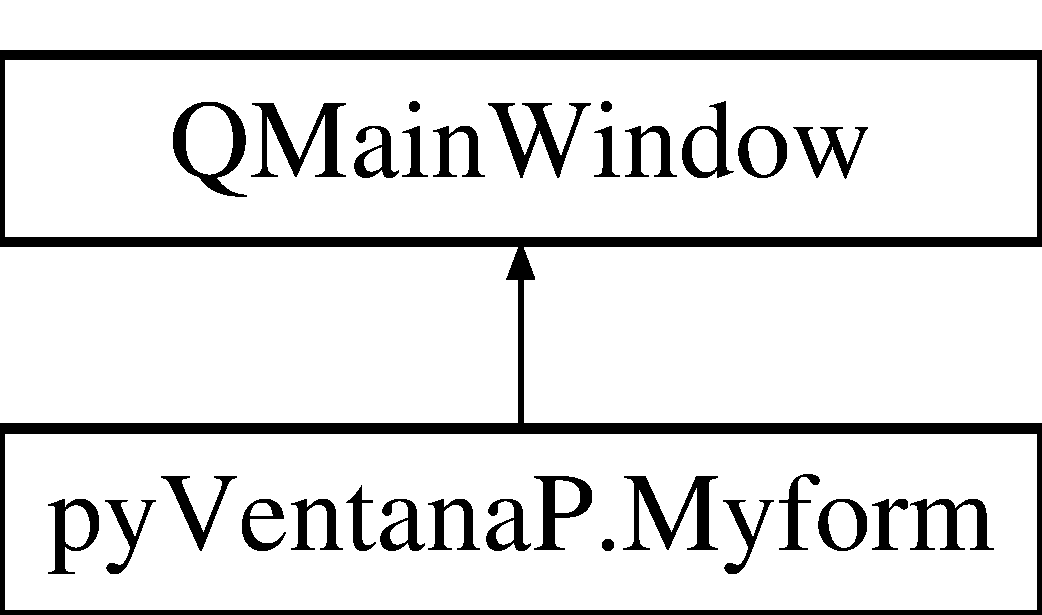
\includegraphics[height=2.000000cm]{classpy_ventana_p_1_1_myform}
\end{center}
\end{figure}
\subsection*{Public Member Functions}
\begin{DoxyCompactItemize}
\item 
\hypertarget{classpy_ventana_p_1_1_myform_a5bcde49821a25bd356dba183ec30e0a2}{def {\bfseries \-\_\-\-\_\-init\-\_\-\-\_\-}}\label{classpy_ventana_p_1_1_myform_a5bcde49821a25bd356dba183ec30e0a2}

\item 
\hypertarget{classpy_ventana_p_1_1_myform_a5f7aa3300f3e72ed75a5b981a4d12c86}{def {\bfseries niveles}}\label{classpy_ventana_p_1_1_myform_a5f7aa3300f3e72ed75a5b981a4d12c86}

\item 
\hypertarget{classpy_ventana_p_1_1_myform_ae43d2fe45766a02dda8dc8c18926d8b5}{def {\bfseries abrir\-Puntajes}}\label{classpy_ventana_p_1_1_myform_ae43d2fe45766a02dda8dc8c18926d8b5}

\item 
def \hyperlink{classpy_ventana_p_1_1_myform_a754fd0296b0df7068ec790267da1df76}{abrir\-Entrar}
\item 
\hypertarget{classpy_ventana_p_1_1_myform_a5718e29c06ffe68c1c34fe16b90d4cf5}{def {\bfseries inicial\-Barra}}\label{classpy_ventana_p_1_1_myform_a5718e29c06ffe68c1c34fe16b90d4cf5}

\item 
\hypertarget{classpy_ventana_p_1_1_myform_a42d99be518114c8a5781a972deabe10f}{def {\bfseries tiempo\-Barra}}\label{classpy_ventana_p_1_1_myform_a42d99be518114c8a5781a972deabe10f}

\end{DoxyCompactItemize}
\subsection*{Public Attributes}
\begin{DoxyCompactItemize}
\item 
\hypertarget{classpy_ventana_p_1_1_myform_a1dfc49b2462b49d9db236f302c4fa79b}{{\bfseries ui}}\label{classpy_ventana_p_1_1_myform_a1dfc49b2462b49d9db236f302c4fa79b}

\item 
\hypertarget{classpy_ventana_p_1_1_myform_a02a5aeacf4313ee916bff8506c4be7ae}{{\bfseries bandera}}\label{classpy_ventana_p_1_1_myform_a02a5aeacf4313ee916bff8506c4be7ae}

\item 
\hypertarget{classpy_ventana_p_1_1_myform_a747dc424bc1e924d538ddaa2c46140fb}{{\bfseries m\-Filename}}\label{classpy_ventana_p_1_1_myform_a747dc424bc1e924d538ddaa2c46140fb}

\item 
\hypertarget{classpy_ventana_p_1_1_myform_a2c41b7f8edd6e28bed342b38585684d5}{{\bfseries m\-File}}\label{classpy_ventana_p_1_1_myform_a2c41b7f8edd6e28bed342b38585684d5}

\item 
\hypertarget{classpy_ventana_p_1_1_myform_a0b1c08087651702d3bbc65fc7fa72c4c}{{\bfseries txtstr}}\label{classpy_ventana_p_1_1_myform_a0b1c08087651702d3bbc65fc7fa72c4c}

\item 
\hypertarget{classpy_ventana_p_1_1_myform_a7d48e6a0b71ab5817fcd051f49f72355}{{\bfseries datos\-Sudoku}}\label{classpy_ventana_p_1_1_myform_a7d48e6a0b71ab5817fcd051f49f72355}

\item 
\hypertarget{classpy_ventana_p_1_1_myform_ab81e63027c7f03d5c4f5c17762bd759b}{{\bfseries valores}}\label{classpy_ventana_p_1_1_myform_ab81e63027c7f03d5c4f5c17762bd759b}

\item 
\hypertarget{classpy_ventana_p_1_1_myform_af181cdbb05c5bed0460017f2ac9d7c63}{{\bfseries nom\-Jugador}}\label{classpy_ventana_p_1_1_myform_af181cdbb05c5bed0460017f2ac9d7c63}

\item 
\hypertarget{classpy_ventana_p_1_1_myform_ae964dc83c3433abcc46f228f31877a11}{{\bfseries nivel\-C}}\label{classpy_ventana_p_1_1_myform_ae964dc83c3433abcc46f228f31877a11}

\item 
\hypertarget{classpy_ventana_p_1_1_myform_a1416abef82a7072feb4e96a4a8d2cadf}{{\bfseries crono}}\label{classpy_ventana_p_1_1_myform_a1416abef82a7072feb4e96a4a8d2cadf}

\item 
\hypertarget{classpy_ventana_p_1_1_myform_af4215ba96d59635495152a476148343b}{{\bfseries timer}}\label{classpy_ventana_p_1_1_myform_af4215ba96d59635495152a476148343b}

\item 
\hypertarget{classpy_ventana_p_1_1_myform_a93db7ad3d0bb6db339f7f0167d99a901}{{\bfseries valor}}\label{classpy_ventana_p_1_1_myform_a93db7ad3d0bb6db339f7f0167d99a901}

\item 
\hypertarget{classpy_ventana_p_1_1_myform_a681584860fb2e817e2d6709c5dd0dae5}{{\bfseries nombre}}\label{classpy_ventana_p_1_1_myform_a681584860fb2e817e2d6709c5dd0dae5}

\item 
\hypertarget{classpy_ventana_p_1_1_myform_ae031463b69e88f85b591ef4355949fe3}{{\bfseries nivel}}\label{classpy_ventana_p_1_1_myform_ae031463b69e88f85b591ef4355949fe3}

\item 
\hypertarget{classpy_ventana_p_1_1_myform_ac7e3ec7dde29a11955ccc15e00393d6b}{{\bfseries principal}}\label{classpy_ventana_p_1_1_myform_ac7e3ec7dde29a11955ccc15e00393d6b}

\end{DoxyCompactItemize}


\subsection{Detailed Description}
\begin{DoxyVerb}@brief funcion init
Instancia la ventana principal de nuestra aplicacion
\end{DoxyVerb}
 

\subsection{Member Function Documentation}
\hypertarget{classpy_ventana_p_1_1_myform_a754fd0296b0df7068ec790267da1df76}{\index{py\-Ventana\-P\-::\-Myform@{py\-Ventana\-P\-::\-Myform}!abrir\-Entrar@{abrir\-Entrar}}
\index{abrir\-Entrar@{abrir\-Entrar}!pyVentanaP::Myform@{py\-Ventana\-P\-::\-Myform}}
\subsubsection[{abrir\-Entrar}]{\setlength{\rightskip}{0pt plus 5cm}def py\-Ventana\-P.\-Myform.\-abrir\-Entrar (
\begin{DoxyParamCaption}
\item[{}]{self}
\end{DoxyParamCaption}
)}}\label{classpy_ventana_p_1_1_myform_a754fd0296b0df7068ec790267da1df76}
\begin{DoxyVerb}@brief funcion abrirPuntajes
Carga los mejores puntajes
\end{DoxyVerb}
\begin{DoxyVerb}@brief funcion abrirEntrar
Nos permite abrir nuestra ventana principal de sudoku
\end{DoxyVerb}
 

The documentation for this class was generated from the following file\-:\begin{DoxyCompactItemize}
\item 
py\-Ventana\-P.\-py\end{DoxyCompactItemize}

\hypertarget{classpy_cargar_s_1_1_myform_cargar_sudoku}{\section{py\-Cargar\-S.\-Myform\-Cargar\-Sudoku Class Reference}
\label{classpy_cargar_s_1_1_myform_cargar_sudoku}\index{py\-Cargar\-S.\-Myform\-Cargar\-Sudoku@{py\-Cargar\-S.\-Myform\-Cargar\-Sudoku}}
}
Inheritance diagram for py\-Cargar\-S.\-Myform\-Cargar\-Sudoku\-:\begin{figure}[H]
\begin{center}
\leavevmode
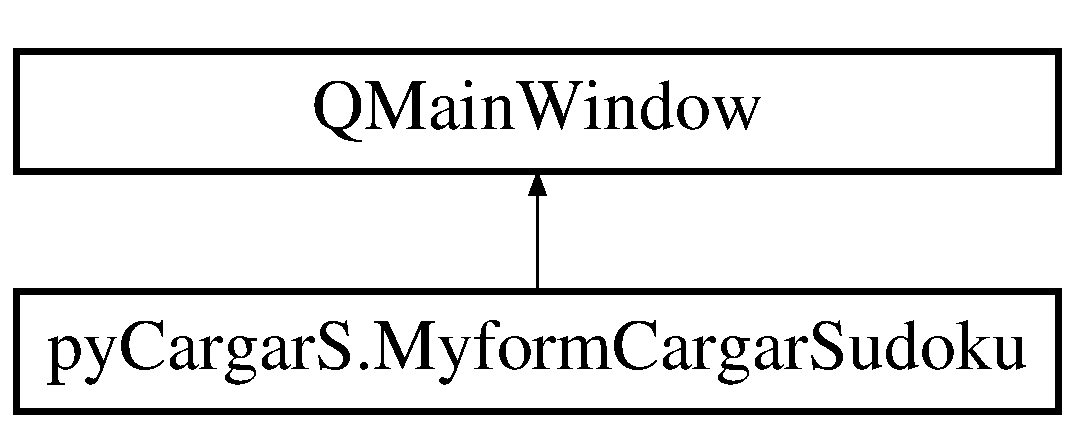
\includegraphics[height=2.000000cm]{classpy_cargar_s_1_1_myform_cargar_sudoku}
\end{center}
\end{figure}


\subsection{Detailed Description}
\begin{DoxyVerb}@brief MyformCargarSudoku
    Invoca una ventana que nos permite cargar una partida
\end{DoxyVerb}
 

The documentation for this class was generated from the following file\-:\begin{DoxyCompactItemize}
\item 
py\-Cargar\-S.\-py\end{DoxyCompactItemize}

\hypertarget{classpy_puntajes_1_1_myform_puntaje}{\section{py\-Puntajes.\-Myform\-Puntaje Class Reference}
\label{classpy_puntajes_1_1_myform_puntaje}\index{py\-Puntajes.\-Myform\-Puntaje@{py\-Puntajes.\-Myform\-Puntaje}}
}
Inheritance diagram for py\-Puntajes.\-Myform\-Puntaje\-:\begin{figure}[H]
\begin{center}
\leavevmode
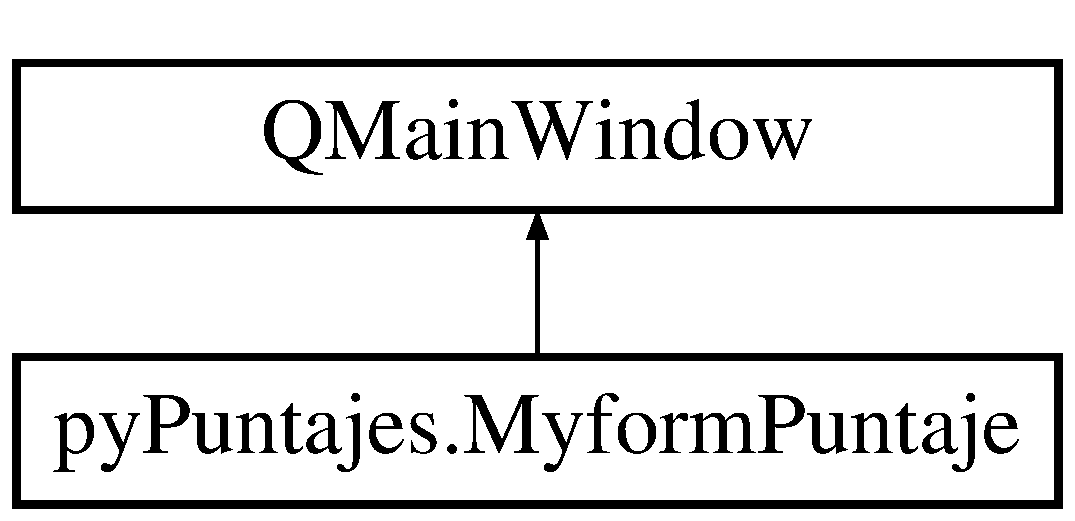
\includegraphics[height=2.000000cm]{classpy_puntajes_1_1_myform_puntaje}
\end{center}
\end{figure}
\subsection*{Public Member Functions}
\begin{DoxyCompactItemize}
\item 
\hypertarget{classpy_puntajes_1_1_myform_puntaje_a494f3dad0f72dec76b44463c06da2b7c}{def {\bfseries \-\_\-\-\_\-init\-\_\-\-\_\-}}\label{classpy_puntajes_1_1_myform_puntaje_a494f3dad0f72dec76b44463c06da2b7c}

\item 
\hypertarget{classpy_puntajes_1_1_myform_puntaje_a2cab2c6564cd5aac0d4a81c9f7ccb11c}{def {\bfseries set\-Puntajes}}\label{classpy_puntajes_1_1_myform_puntaje_a2cab2c6564cd5aac0d4a81c9f7ccb11c}

\item 
\hypertarget{classpy_puntajes_1_1_myform_puntaje_a87541d36caacfbecc554dc915e812f2b}{def {\bfseries set\-Ventana\-Principal}}\label{classpy_puntajes_1_1_myform_puntaje_a87541d36caacfbecc554dc915e812f2b}

\item 
\hypertarget{classpy_puntajes_1_1_myform_puntaje_a33ec28b841e9f14570491bbbc0a2ba05}{def {\bfseries volver\-Ventana}}\label{classpy_puntajes_1_1_myform_puntaje_a33ec28b841e9f14570491bbbc0a2ba05}

\end{DoxyCompactItemize}
\subsection*{Public Attributes}
\begin{DoxyCompactItemize}
\item 
\hypertarget{classpy_puntajes_1_1_myform_puntaje_ad0ef16ab536e79217ba54114f6d38710}{{\bfseries ui\-P}}\label{classpy_puntajes_1_1_myform_puntaje_ad0ef16ab536e79217ba54114f6d38710}

\item 
\hypertarget{classpy_puntajes_1_1_myform_puntaje_a95c48840e765e45dff549cb05b2315c5}{{\bfseries m\-Filename}}\label{classpy_puntajes_1_1_myform_puntaje_a95c48840e765e45dff549cb05b2315c5}

\item 
\hypertarget{classpy_puntajes_1_1_myform_puntaje_a84d84248f4d6f892bccde7f61d175149}{{\bfseries m\-File}}\label{classpy_puntajes_1_1_myform_puntaje_a84d84248f4d6f892bccde7f61d175149}

\item 
\hypertarget{classpy_puntajes_1_1_myform_puntaje_a7fdcaed39668e056fba3ff7f0830b539}{{\bfseries txtstr}}\label{classpy_puntajes_1_1_myform_puntaje_a7fdcaed39668e056fba3ff7f0830b539}

\item 
\hypertarget{classpy_puntajes_1_1_myform_puntaje_a98442c05fa83ff85a39e09b5d6027cfe}{{\bfseries datos\-Sudoku}}\label{classpy_puntajes_1_1_myform_puntaje_a98442c05fa83ff85a39e09b5d6027cfe}

\item 
\hypertarget{classpy_puntajes_1_1_myform_puntaje_a0422b673c26422eafd94db1ee01006cf}{{\bfseries valores}}\label{classpy_puntajes_1_1_myform_puntaje_a0422b673c26422eafd94db1ee01006cf}

\item 
\hypertarget{classpy_puntajes_1_1_myform_puntaje_ac37b988b49ecf558cdf3e1da00b52b4b}{{\bfseries nom\-Jugador}}\label{classpy_puntajes_1_1_myform_puntaje_ac37b988b49ecf558cdf3e1da00b52b4b}

\item 
\hypertarget{classpy_puntajes_1_1_myform_puntaje_a6dd3e2825a1e17788aa5f6e59dbdc774}{{\bfseries nivel\-C}}\label{classpy_puntajes_1_1_myform_puntaje_a6dd3e2825a1e17788aa5f6e59dbdc774}

\item 
\hypertarget{classpy_puntajes_1_1_myform_puntaje_a9bab9e37f4460c08b4b17c0cf992e7ec}{{\bfseries crono}}\label{classpy_puntajes_1_1_myform_puntaje_a9bab9e37f4460c08b4b17c0cf992e7ec}

\item 
\hypertarget{classpy_puntajes_1_1_myform_puntaje_a5d14fae0189ad9ab4b388814d6a1059b}{{\bfseries valor\-C}}\label{classpy_puntajes_1_1_myform_puntaje_a5d14fae0189ad9ab4b388814d6a1059b}

\item 
\hypertarget{classpy_puntajes_1_1_myform_puntaje_af581fe4c19624a75a8929ad70d8dd7a2}{{\bfseries min}}\label{classpy_puntajes_1_1_myform_puntaje_af581fe4c19624a75a8929ad70d8dd7a2}

\item 
\hypertarget{classpy_puntajes_1_1_myform_puntaje_a8d5cf012b41f172b5a123c0b86106cb0}{{\bfseries seg}}\label{classpy_puntajes_1_1_myform_puntaje_a8d5cf012b41f172b5a123c0b86106cb0}

\item 
\hypertarget{classpy_puntajes_1_1_myform_puntaje_a8a0076112eab8b0579a2f69c38d7de41}{{\bfseries mseg}}\label{classpy_puntajes_1_1_myform_puntaje_a8a0076112eab8b0579a2f69c38d7de41}

\item 
\hypertarget{classpy_puntajes_1_1_myform_puntaje_a7d1817b346dacfed67ee8473a5424c78}{{\bfseries puntaje}}\label{classpy_puntajes_1_1_myform_puntaje_a7d1817b346dacfed67ee8473a5424c78}

\item 
\hypertarget{classpy_puntajes_1_1_myform_puntaje_ae7244b25eaeb79977827f7acbacf3fb8}{{\bfseries strc}}\label{classpy_puntajes_1_1_myform_puntaje_ae7244b25eaeb79977827f7acbacf3fb8}

\item 
\hypertarget{classpy_puntajes_1_1_myform_puntaje_a61090f0911b38c693f23d928780a32cd}{{\bfseries principal}}\label{classpy_puntajes_1_1_myform_puntaje_a61090f0911b38c693f23d928780a32cd}

\end{DoxyCompactItemize}


\subsection{Detailed Description}
\begin{DoxyVerb}@brief funcion init
Muestra la ventana de puntaje
\end{DoxyVerb}
 

The documentation for this class was generated from the following file\-:\begin{DoxyCompactItemize}
\item 
py\-Puntajes.\-py\end{DoxyCompactItemize}

\hypertarget{classpy_sudoku_1_1_myform_sudoku}{\section{py\-Sudoku.\-Myform\-Sudoku Class Reference}
\label{classpy_sudoku_1_1_myform_sudoku}\index{py\-Sudoku.\-Myform\-Sudoku@{py\-Sudoku.\-Myform\-Sudoku}}
}
Inheritance diagram for py\-Sudoku.\-Myform\-Sudoku\-:\begin{figure}[H]
\begin{center}
\leavevmode
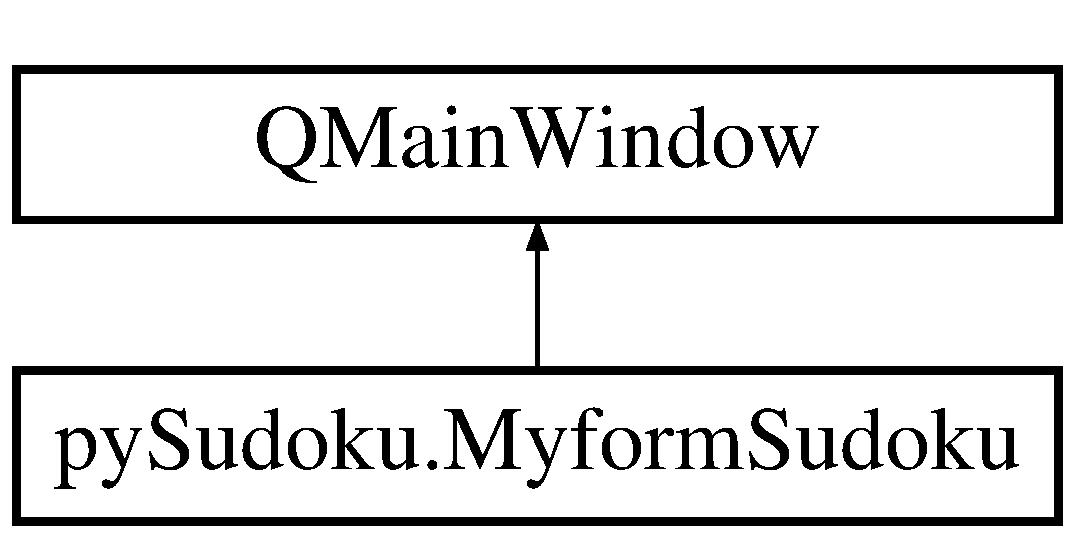
\includegraphics[height=2.000000cm]{classpy_sudoku_1_1_myform_sudoku}
\end{center}
\end{figure}


\subsection{Detailed Description}
\begin{DoxyVerb}@brief Funcion Main de Pysudoku
Esta funcion concta las se�ales con los procesos y llama a la funcion que crea el tablero del juego
\end{DoxyVerb}
 

The documentation for this class was generated from the following file\-:\begin{DoxyCompactItemize}
\item 
py\-Sudoku.\-py\end{DoxyCompactItemize}

%--- End generated contents ---

% Index
\newpage
\phantomsection
\addcontentsline{toc}{part}{Index}
\printindex

\end{document}
